\chapter{系统需求分析}

\section{业务需求分析}
\subsection{用户角色定义}
本系统的业务目标是把用户提交的自然语言需求转换为可预览、可保存和可下载的 Vue 3 单文件组件。结合当前代码，系统已经形成账号登录、项目空间、生成任务、版本记录、用量控制和管理员治理的完整链路。本章的需求分析以这些已经落地的能力为边界展开。

普通用户是系统的主要使用者。用户登录后创建或切换项目空间，填写组件名称、需求描述和约束信息，随后发起组件生成任务，查看历史版本，并下载生成结果。管理员承担系统治理职责，负责用户检索、角色调整、账号启停和审计日志查看。软件工程中的模型任务通常依赖完整的环境接口和状态反馈，而不只是模型本身的输出（SWE-agent: Agent-Computer Interfaces Enable Automated Software Engineering）\cite{yang2024sweagent}。

\begin{table}[htbp]
\centering
\caption{系统角色与业务边界}
\label{tab:chapter3-roles}
\small
\begin{tabular}{@{}p{0.18\textwidth}p{0.25\textwidth}p{0.35\textwidth}p{0.12\textwidth}@{}}
\toprule
角色 & 业务目标 & 主要业务活动 & 权限边界 \\
\midrule
普通用户 & 完成组件生成、确认结果可用并形成下载文件 & 登录系统、选择项目、提交组件需求、查看生成结果、预览与下载版本、查看用量信息 & 本人账号与本人项目 \\
管理员 & 维护系统账号秩序并支持事后追踪 & 查询用户、调整角色、启停账号、查看审计日志 & 管理接口与审计数据 \\
\bottomrule
\end{tabular}
\end{table}

表 \ref{tab:chapter3-roles} 体现了本系统的参与者划分。需求分析阶段更关注各类参与者要完成什么业务、系统需要为其提供什么边界条件，而不是直接展开到具体类和接口。权限控制、项目隔离和审计记录都服务于这一业务边界。

\subsection{业务流程建模}
业务流程从登录和项目选择开始，经过任务创建、生成执行、结构化抽取、安全校验、版本保存和在线交付。前端请求会携带会话令牌和项目标识，后端据此恢复当前用户并定位项目范围。生成开始前，系统会检查当日 token 额度，并尝试读取缓存。未命中缓存时，后端通过 SSE 返回流式生成片段；命中缓存时，系统直接生成版本结果并返回。

模型输出不会直接进入预览。后端需要先抽取 \texttt{template}、\texttt{script} 和 \texttt{style}，再进行安全扫描。若检测到阻断级风险，任务会被标记为失败并返回原因；若扫描通过，系统保存版本与调用日志，供后续预览、下载和用量统计使用。端到端任务链路中的状态管理和结果校验会直接影响结果能否复现和定位（SWE-bench: Can Language Models Resolve Real-World GitHub Issues?）\cite{jimenez2024swebench}。

\begin{figure}[!htbp]
\centering
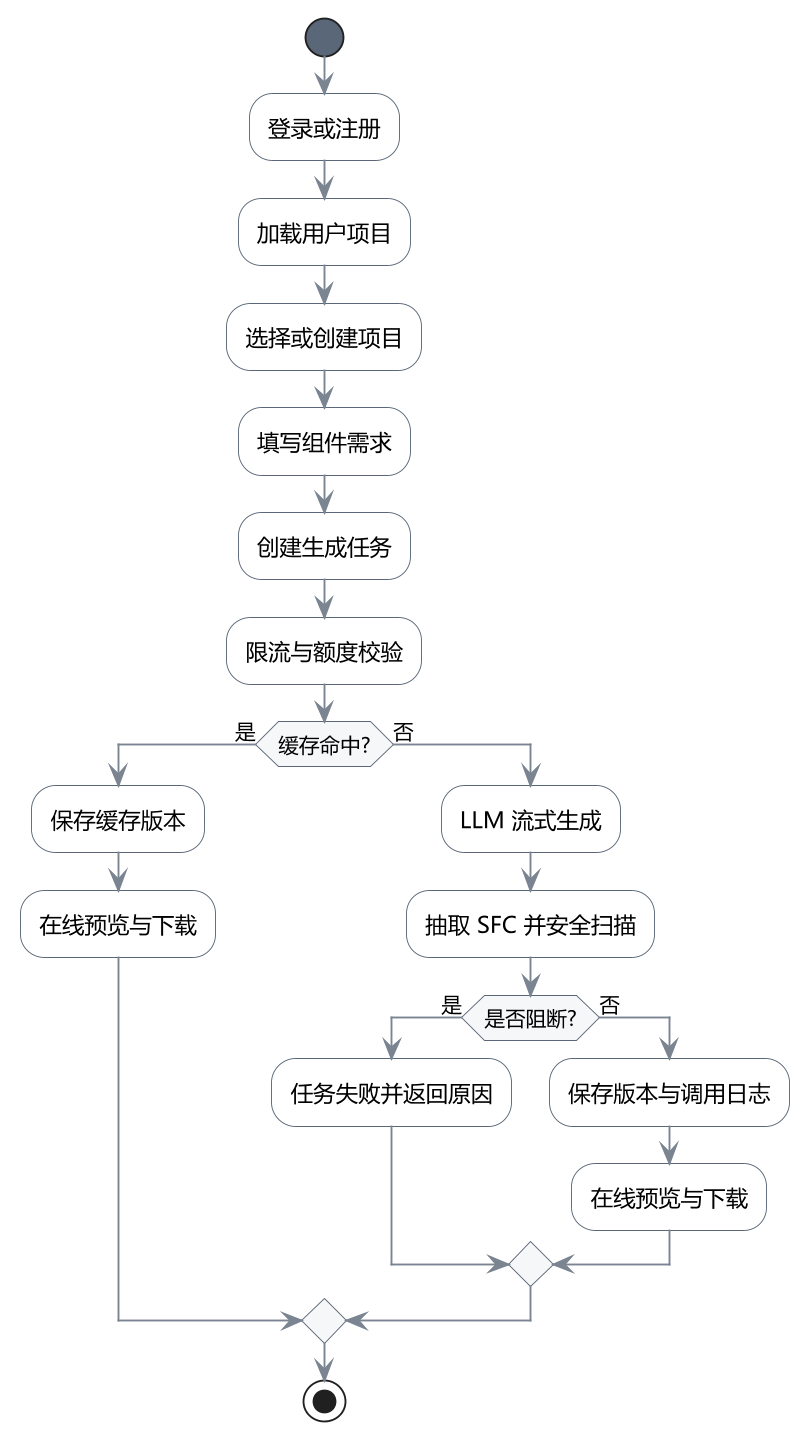
\includegraphics[width=0.34\textwidth,height=0.78\textheight,keepaspectratio]{figures/chapter3-flow-plantuml.png}
\caption{业务活动流程图}
\label{fig:chapter3-flow}
\end{figure}

\vspace{-0.25em}

\begin{table}[htbp]
\centering
\caption{业务流程关键节点与实现依据}
\label{tab:chapter3-flow-io}
\small
\begin{tabular}{@{}p{0.18\textwidth}p{0.32\textwidth}p{0.40\textwidth}@{}}
\toprule
流程节点 & 输入要素 & 当前实现输出 \\
\midrule
登录与会话 & 用户名、密码 & 会话令牌、用户编号、角色、过期时间 \\
项目选择 & 当前用户、项目名称或项目编号 & 项目记录、工作区记录、请求头项目标识 \\
任务创建 & 组件名称、需求描述、约束条件 & 任务编号、任务状态、所属项目关系 \\
生成执行 & 任务编号、模型配置、系统提示词 & token 流、缓存命中标记、完成或错误事件 \\
安全与版本 & 模型输出、SFC 抽取结果 & 安全等级、版本编号、可下载组件代码 \\
管理审计 & 管理员操作、目标用户 & 审计日志、角色或账号状态变更结果 \\
\bottomrule
\end{tabular}
\end{table}

\section{功能需求分析}
\subsection{用例图及用例描述}
功能需求分析需要从用户完成任务的过程出发，而不是从代码模块出发。图 \ref{fig:chapter3-usecase} 展示了系统面向普通用户与管理员的主用例。普通用户侧重点在注册登录、生成组件代码、在线预览、下载文件以及项目与版本管理，管理员侧重点在用户查询、权限更改、账号启停和日志查看。图中只保留主用例层级，用于说明系统对外提供的功能边界；更细的操作条件和结果再通过表格展开描述。

\begin{figure}[!htbp]
\centering
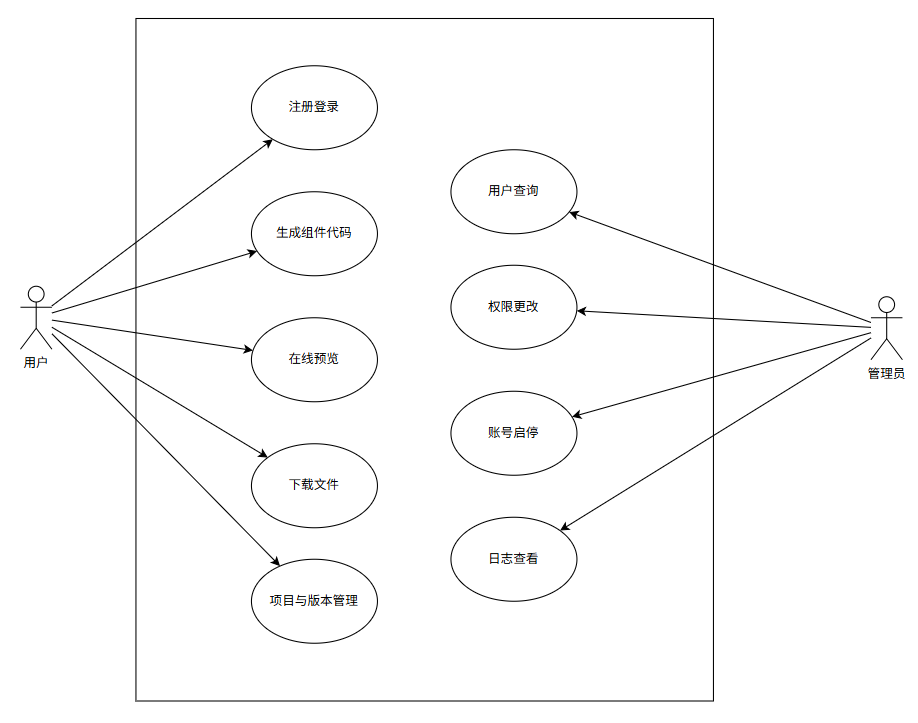
\includegraphics[width=0.94\textwidth,height=0.46\textheight,keepaspectratio]{figures/用例图.png}
\caption{系统核心用例图}
\label{fig:chapter3-usecase}
\end{figure}

\vspace{-0.2em}

普通用户的核心用例围绕一次组件生成任务展开。用户进入系统后，需要先完成注册或登录，然后在个人项目范围内创建新项目或切换已有项目。项目选定后，用户提交组件名称、自然语言描述和约束条件，系统进入生成阶段并持续返回进度信息。生成完成后，用户可以在页面中直接预览结果，也可以下载版本文件，并在项目与版本管理功能中回看同一项目下已经保存的任务和版本。

管理员的核心用例主要用于系统治理。管理员可以查询当前用户及账号状态，必要时更改权限或启停账号，也可以查看日志以追踪关键管理操作。为了避免用例图承载过多细节，表 \ref{tab:chapter3-modules} 在主用例的基础上进一步说明前置条件和业务结果。

\begin{table}[!htbp]
\centering
\caption{核心用例描述}
\label{tab:chapter3-modules}
\small
\begin{tabular}{@{}p{0.18\textwidth}p{0.14\textwidth}p{0.26\textwidth}p{0.28\textwidth}@{}}
\toprule
用例名称 & 参与者 & 前置条件 & 结果 \\
\midrule
注册与登录 & 普通用户 & 用户尚未进入系统或当前会话已失效 & 系统建立有效登录状态，允许进入个人项目空间 \\
项目管理 & 普通用户 & 用户已经登录 & 系统确定当前项目范围，后续任务和历史记录都归入该项目 \\
组件生成 & 普通用户 & 用户已经登录并选定项目 & 系统创建生成任务，进入流式生成阶段 \\
结果查看 & 普通用户 & 生成任务已经创建 & 用户看到增量结果、完成状态或失败原因，系统记录调用信息 \\
在线预览与下载版本 & 普通用户 & 已经生成可用版本 & 用户确认结果并获取可交付的组件文件 \\
查询历史任务与版本 & 普通用户 & 当前项目下已存在历史任务 & 用户能够回看历史结果并选择指定版本 \\
用量查看 & 普通用户 & 用户已经登录 & 用户能够查看当日 token 使用量、估算费用和剩余额度 \\
用户治理与审计 & 管理员 & 管理员已登录 & 管理员能够完成用户查询、角色调整、账号启停和审计记录查看 \\
\bottomrule
\end{tabular}
\end{table}

\vspace{-0.25em}

\section{非功能需求分析}
\subsection{性能指标}
本系统的性能需求集中在普通接口响应和生成过程反馈两个方面。登录、项目查询、历史任务、版本详情、用量查询和管理员用户列表属于普通 HTTP 接口，应保持较快响应。组件生成依赖第三方模型服务，整体耗时受模型推理影响较大，因此系统采用 SSE 返回增量内容，让用户在等待期间持续获得反馈，而不是长时间无响应。

并发场景下，系统需要保证任务状态、版本数据和调用日志的一致性。当前做法是把任务、版本和日志持久化到数据库，同时使用内存缓存减少重复生成和短时间统计查询。这样的设计适合当前单体应用。若缺少任务状态和调用记录，模型辅助生成场景中的问题很难定位到输入、模型响应还是后处理阶段（SWE-bench: Can Language Models Resolve Real-World GitHub Issues?）\cite{jimenez2024swebench}。

\begin{table}[htbp]
\centering
\caption{非功能需求与当前实现}
\label{tab:chapter3-nonfunctional}
\small
\begin{tabular}{@{}p{0.18\textwidth}p{0.32\textwidth}p{0.40\textwidth}@{}}
\toprule
需求类别 & 目标说明 & 当前实现方式 \\
\midrule
响应体验 & 普通页面快速返回，生成过程可见 & HTTP 接口配合 SSE 流式事件 \\
状态可靠性 & 刷新页面后仍可查询任务和版本 & 任务、版本和调用日志持久化到数据库 \\
成本控制 & 限制用户当日模型消耗 & 额度检查、调用日志、用量缓存 \\
重复请求控制 & 减少相同需求的重复模型调用 & 基于任务内容摘要的内存生成缓存 \\
错误可追踪 & 生成失败可返回明确原因 & 任务状态、错误消息和安全阻断原因入库 \\
管理可审计 & 管理操作留痕 & 管理员操作写入审计日志 \\
\bottomrule
\end{tabular}
\end{table}

\subsection{安全性要求}
安全需求覆盖账号、接口、资源和生成代码。账号安全要求密码不能明文保存，当前后端使用 BCrypt 保存密码哈希。接口安全要求系统能够识别合法登录状态，当前后端通过会话令牌和 \texttt{user\_session} 表恢复用户身份。资源安全要求普通用户只能访问自己的项目、任务和版本，管理员接口只能由管理员调用，这部分由 \texttt{AuthInterceptor}、\texttt{AuthContextHolder} 和 \texttt{AuthorizationService} 共同完成。

生成代码安全要求模型输出在进入预览和下载之前经过检查。当前后端在版本保存前执行安全扫描，前端预览前再做一次检测，从而降低高风险代码进入运行环境的可能性。安全开发框架强调风险控制应尽量前移到设计和实现阶段（Secure Software Development Framework (SSDF) Version 1.1）\cite{nistssdf2024}。常见弱点治理研究也提示应重点关注危险执行、输入边界和不受控资源访问（CWE Top 25 Most Dangerous Software Weaknesses）\cite{cwe2024top25}。

表 \ref{tab:chapter3-security} 对本系统当前的安全需求与控制措施进行了归纳。账号密码、接口会话、资源归属、管理接口和生成代码是本项目中最需要前置控制的几个风险点。

\begin{table}[htbp]
\centering
\caption{安全需求与当前控制措施}
\label{tab:chapter3-security}
\small
\begin{tabular}{@{}p{0.20\textwidth}p{0.34\textwidth}p{0.36\textwidth}@{}}
\toprule
安全对象 & 需求说明 & 当前控制措施 \\
\midrule
账号密码 & 避免明文保存密码 & BCrypt 哈希保存与登录校验 \\
接口会话 & 阻止未登录访问业务接口 & \texttt{X-Auth-Token}、\texttt{user\_session}、拦截器 \\
资源归属 & 防止访问他人项目和任务 & 当前用户上下文、项目拥有者关系 \\
管理接口 & 限制普通用户调用管理功能 & \texttt{ADMIN} 角色与权限枚举校验 \\
生成代码 & 阻断高风险组件代码 & 后端安全扫描与前端预览前检测 \\
管理行为 & 保存关键管理操作记录 & \texttt{audit\_log} 审计日志 \\
\bottomrule
\end{tabular}
\end{table}

\subsection{可扩展性设计}
当前系统已经把账号、项目、生成、版本、成本和管理拆分到不同控制器与服务中，模型调用、SFC 抽取、安全扫描、缓存和费用记录也分别由独立组件处理。这种结构有利于在不改变前端主流程的情况下调整模型供应商、提示词模板或安全规则。数据层已经建立用户、项目、任务和版本之间的明确关系，因此后续若增加更多生成元数据或统计字段，也可以围绕现有实体逐步扩展。

\section{可行性分析}
\subsection{技术可行性}
从技术实现看，当前系统采用前后端分离方式。前端负责需求输入、状态展示、预览和下载，后端负责认证授权、任务创建、模型调用、结果处理、持久化和管理接口。Vue 3、Spring Boot、MySQL 和 SSE 能够覆盖本项目的主要业务需求。当前代码已经实现完整的业务闭环，技术风险主要集中在模型服务稳定性、生成代码安全性和长连接异常处理上。项目已经通过缓存、额度检查、安全扫描和错误事件返回对这些问题进行约束。软件工程场景中的模型任务需要环境接口、状态反馈和结果验证共同配合，这一点已经在相关研究中得到说明（SWE-agent: Agent-Computer Interfaces Enable Automated Software Engineering）\cite{yang2024sweagent}。

\subsection{经济可行性}
本系统的开发成本主要来自常规 Web 开发环境和第三方模型调用。前后端框架、数据库和大部分依赖都可以在普通开发设备上运行，不需要额外专用硬件。运行阶段的主要可变成本来自模型 token 消耗，当前系统已经提供 token 统计、费用估算、额度校验和短期缓存，这使系统具备基本的成本控制能力。

\subsection{操作可行性}
普通用户的操作集中在登录、项目选择、需求填写、生成、预览、历史查看和下载，交互路径较短。管理员页面则聚焦用户检索、角色切换、账号启停和审计查看。系统对登录失败、额度不足、生成失败和安全阻断等情况都能返回明确提示，因此用户不需要了解后端实现细节，也能够根据页面反馈完成主要操作。\par




